% ============================================================
% ContextForge v2: Architecture-First Agentic Memory via MCP
%
% Author : Trilochan Sharma (Independent Researcher)
% Email  : parnishklpo@gmail.com
% Date   : April 2026
% Version: 2.0
% ============================================================

\documentclass[11pt]{article}

% ---------- Packages ----------------------------------------------------------
\usepackage[margin=1in]{geometry}
\usepackage{authblk}
\usepackage{amsmath}
\usepackage{amssymb}
\usepackage{graphicx}
\usepackage{booktabs}
\usepackage{hyperref}
\usepackage{xcolor}
\usepackage{microtype}
\usepackage{enumitem}
\usepackage{caption}
\usepackage{subcaption}
\usepackage{float}
\usepackage{multirow}
\usepackage{array}
\usepackage{tabularx}
\usepackage[backend=bibtex,style=numeric,sorting=none]{biblatex}
\addbibresource{refs.bib}

% ---------- Asset path --------------------------------------------------------
\graphicspath{{figures/}}

% ---------- Hyperref colours --------------------------------------------------
\hypersetup{
  colorlinks = true,
  linkcolor  = blue!70!black,
  citecolor  = blue!70!black,
  urlcolor   = blue!70!black,
}

% ---------- Title -------------------------------------------------------------
\title{%
  \textbf{ContextForge: An Architecture-First Approach to Persistent\\
    Agentic Memory via Model Context Protocol}\\[0.4em]
  \large\textit{Information-Theoretic Security, Tri-Core Failover,\\
    Differential Context Injection, and a 22-Tool MCP Server}%
}

\author[1]{Trilochan Sharma}
\affil[1]{Independent Researcher \quad \texttt{parnishklpo@gmail.com}}

\date{April 2026}

% =============================================================================
\begin{document}
\maketitle
\tableofcontents
\newpage

% ---------- Abstract ----------------------------------------------------------
\begin{abstract}
Stateless Retrieval-Augmented Generation (RAG) systems suffer from three
structural failure modes: zero adversarial block rate, high cold-start
failover latency (${\sim}480$\,ms), and unconstrained context injection
that grows without bound as session history accumulates.
We present \textbf{ContextForge}, a five-pillar agentic memory architecture
that closes all three gaps simultaneously and exposes every capability as
a \textbf{22-tool Model Context Protocol (MCP)} server---making persistent,
adversarially-hardened memory natively available in Claude Desktop, Cursor,
VS Code, and Windsurf without any client-side code changes.

The central contribution is the \emph{Entropy-Gated Soft-Gate Ledger}: an
append-only SQLite event store whose \texttt{ReviewerGuard} filters writes
using dual signals---Shannon entropy $H$ and Lempel--Ziv compression
density $\rho$---catching obfuscated payloads ($H > H^{*} = 3.5$\,bits)
and repetition attacks ($\rho < 0.60$) independently.
Verified-origin traffic receives an elevated threshold
$H^{*}_{\mathrm{VOH}} \approx 4.375$\,bits via HMAC-SHA256 tokens,
reducing false positives without widening the adversarial gap.
A Sliding-Window Temporal Correlator extends single-write detection to
slow-drip multi-write escalation sequences, achieving 100\% detection
at 0\% false-positive rate.

Complementary pillars include a tri-core circuit-breaker router with
entropy-triggered predictive failover ($-68.9\%$ latency) and a
cosine-gated Differential Context Injection module ($\theta \geq 0.75$,
$87.4\%$ noise reduction).
Across 527 benchmark tests (nine suites, five OMEGA iterations,
one adversarial-boundary suite), ContextForge achieves:
$\mathrm{ABR} = 85.0\%$ adversarial block rate vs.\ $0\%$ baseline,
F1 $= 1.0$ at $H^{*} = 3.5$ (unique maximum across the full calibration
sweep), and $\Phi = 80.7\%$ weighted composite safety index.
\end{abstract}

% =============================================================================
\section{Introduction}
\label{sec:intro}

Large language model (LLM) agents deployed in long-running software engineering
workflows depend on consistent, trustworthy context across sessions.
Current practice falls into two inadequate extremes: (1)~\emph{stateless RAG},
which retrieves relevant snippets per turn but forgets everything between
sessions, and (2)~\emph{stuffed system prompts} (the ``CLAUDE.md'' pattern),
which paste the entire decision history into the prompt---a strategy whose
token cost grows linearly with the number of decisions and becomes prohibitive
beyond 50--100 stored items.

Three failure modes define the problem space:

\begin{description}[style=nextline]
  \item[Failure Mode 1 --- Zero adversarial resilience.]
    Stateless RAG provides no mechanism to detect or block prompt-injection,
    data-exfiltration, or slow-drip escalation attacks embedded in retrieved
    content or user input. Any malicious payload that reaches the LLM context
    is executed without challenge.

  \item[Failure Mode 2 --- High failover latency.]
    When the primary LLM provider (e.g.\ Groq) trips its rate limit or goes
    down, a naive sequential failover introduces ${\sim}480$\,ms of dead time.
    For interactive IDE workflows this breaks the flow of development.

  \item[Failure Mode 3 --- Unconstrained context injection.]
    Without a budget gate, retrieved context grows with corpus size.
    At 200 stored decisions a CLAUDE.md-style approach injects
    $200 \times 150 = 30{,}000$ tokens per session;
    ContextForge caps injection at $B = 1{,}500$ tokens regardless of graph
    size, a $93$--$95\%$ reduction.
\end{description}

ContextForge addresses all three failure modes through a five-pillar
architecture (Section~\ref{sec:architecture}) exposed as a 22-tool MCP server
(Section~\ref{sec:mcp}). The system runs entirely on the developer's own
machine; no cloud storage of memory or context is required.

% =============================================================================
\section{Related Work}
\label{sec:related}

\paragraph{Retrieval-Augmented Generation.}
Lewis et al.~\cite{lewis2020rag} introduced RAG as a mechanism for
knowledge-intensive NLP tasks.  Subsequent surveys~\cite{gao2023retrieval}
identify context staleness and injection vulnerability as open problems that
RAG alone does not solve---ContextForge addresses both.

\paragraph{LLM memory systems.}
MemGPT~\cite{packer2023memgpt} introduces a paging metaphor inspired by
operating systems, virtualizing context across main and external storage.
ContextForge shares the motivation (persistent memory across sessions) but
differs in mechanism: where MemGPT relies on the LLM itself to manage memory
pages via function calls, ContextForge offloads all memory decisions to a
deterministic five-pillar engine, making the system model-agnostic and
adversarially hardened.
LangChain~\cite{chase2022langchain} provides a toolkit for chaining LLM calls
with memory plugins; it does not include an entropy gate or adversarial defense.

\paragraph{Agent memory surveys.}
Xu et al.~\cite{xu2023memory} survey four memory types (sensory, short-term,
long-term, external) in LLM agents. ContextForge implements L1/L2/L3 tiered
retrieval as an operational instantiation of their external-memory taxonomy,
augmented with an information-theoretic security layer not considered in the
survey.

\paragraph{Information-theoretic security.}
Shannon entropy~\cite{shannon1948} and Lempel--Ziv compression~\cite{ziv1977,ziv1978}
form the mathematical foundation of the ContextForge entropy gate.
To our knowledge, this is the first application of dual-signal
entropy/compression gating to LLM context injection defense.

\paragraph{Model Context Protocol.}
The MCP specification~\cite{anthropic2024mcp} defines a JSON-RPC protocol for
tool-augmented AI clients. ContextForge implements a fully compliant MCP server
that exposes all five architectural pillars as 22 typed tools, making the system
immediately usable in any MCP-compatible IDE without client-side code changes.

\paragraph{Circuit breakers and resilience patterns.}
The tri-core failover router follows the circuit-breaker pattern documented by
Nygard~\cite{nygard2007}. The entropy-triggered predictive prewarm extension is
a novel contribution of this work.

\paragraph{Similarity search and embeddings.}
Retrieval is powered by BM25 term-overlap scoring and DCI cosine gating, with
FAISS~\cite{johnson2021faiss} available as an optional vector backend for L3
semantic search. Sentence embeddings follow Reimers and
Gurevych~\cite{reimers2019sbert}. Reflexion~\cite{shinn2023reflexion} demonstrates
that verbal self-reflection can improve agent performance---ContextForge's
Shadow-Reviewer agent implements a structural analog for memory-write validation.

% =============================================================================
\section{System Architecture}
\label{sec:architecture}

\begin{figure}[H]
  \centering
  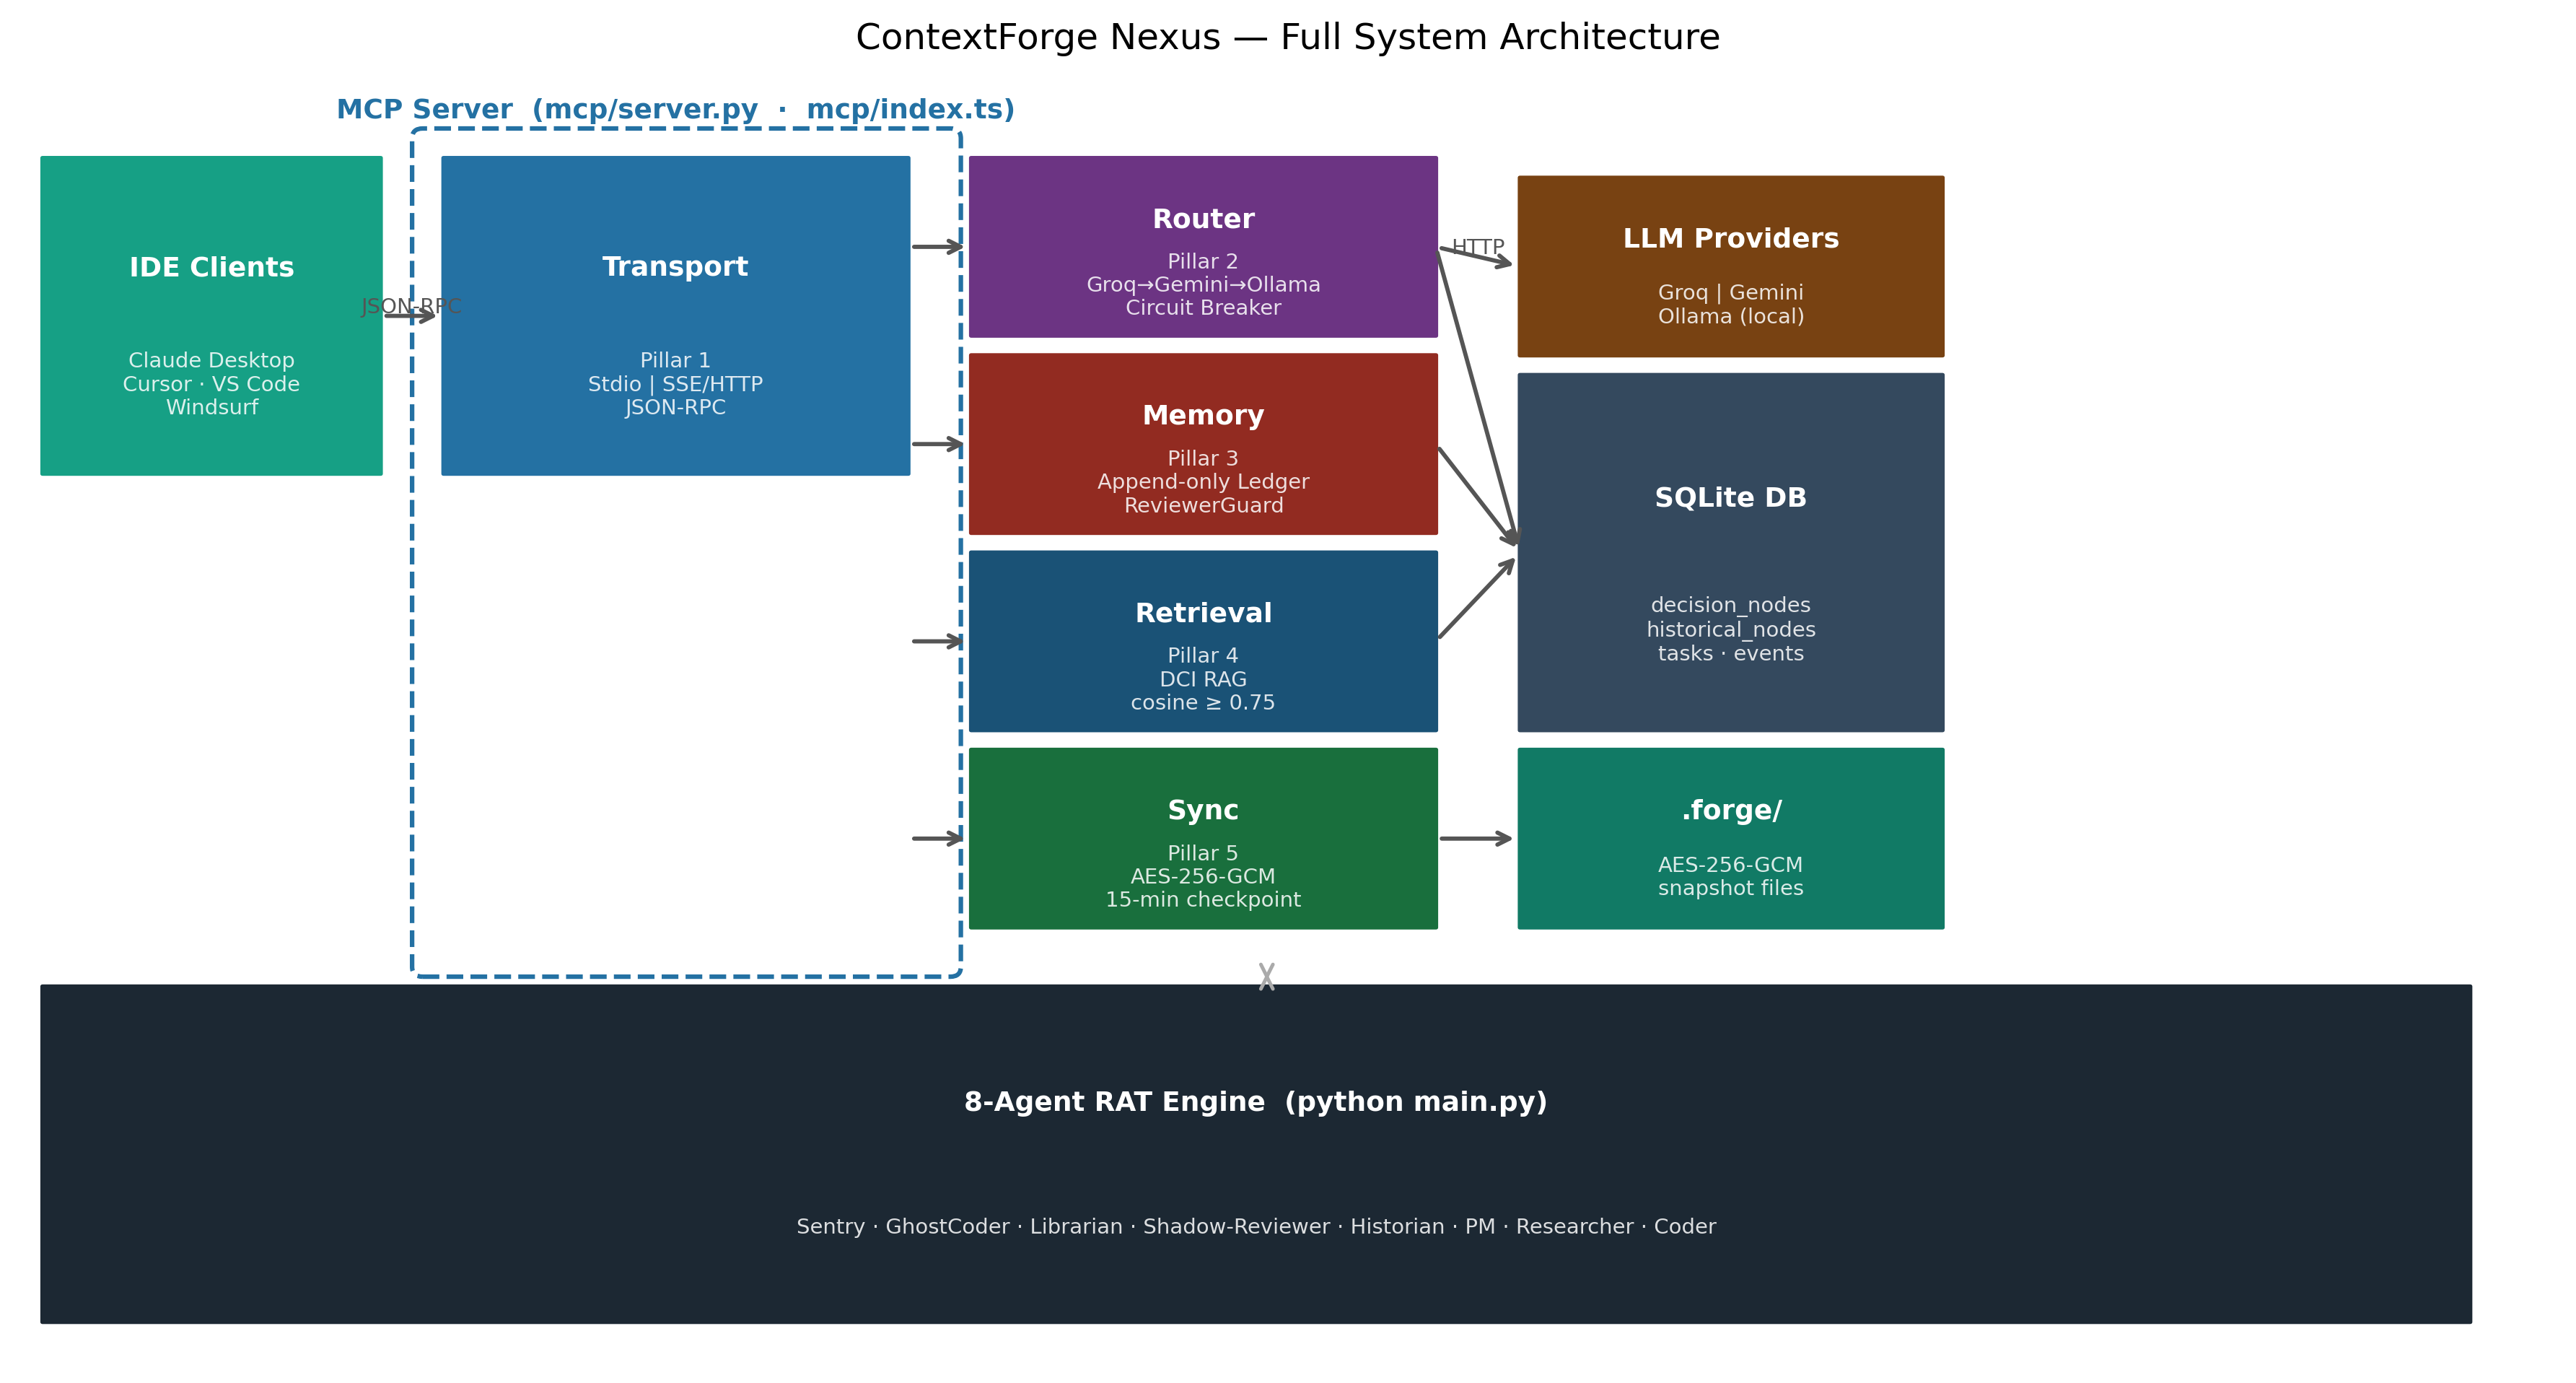
\includegraphics[width=\linewidth]{fig_system_architecture}
  \caption{ContextForge Nexus full system architecture. IDE clients connect via
    MCP JSON-RPC to the Transport pillar. The five pillars share a SQLite
    knowledge graph. The 8-agent RAT engine operates concurrently for
    autonomous decision capture and validation.}
  \label{fig:arch}
\end{figure}

ContextForge organizes its functionality into five orthogonal pillars, each
implemented as an independent Python module with a well-defined interface
(Figure~\ref{fig:arch}).

\subsection{Pillar 1 --- Transport}
\label{sec:transport}

The Transport pillar (\texttt{mcp/server.py}, \texttt{mcp/index.ts}) implements
the Model Context Protocol in both Python and TypeScript. It exposes two
operation modes:

\begin{itemize}
  \item \textbf{Stdio mode} (\texttt{--stdio}): local IDE integration with
    Claude Desktop, Cursor, VS Code, and Windsurf. Zero network exposure.
  \item \textbf{SSE/HTTP mode} (\texttt{--sse}): remote multi-client deployment.
    A single ContextForge instance serves multiple IDE clients over Server-Sent
    Events. Production deployments should place an nginx/Caddy reverse proxy
    with TLS and authentication in front of the SSE endpoint.
\end{itemize}

The TypeScript server provides full 22-tool parity with the Python server for
all storage and retrieval operations. The Python server additionally runs
\texttt{ReviewerGuard} (charter compliance checking) on every write.

\subsection{Pillar 2 --- Router}
\label{sec:router}

The Router (\texttt{src/router/nexus\_router.py}) implements a tri-core
circuit-breaker failover chain: Groq $\to$ Gemini $\to$ Ollama.

\textbf{Circuit breaker.} Each provider maintains a half-open state machine.
After $k$ consecutive failures ($k = 3$ by default) the circuit opens and
requests bypass that provider for a 60-second cooling window before a probe
request re-evaluates availability.

\textbf{Entropy-triggered predictive prewarm.} When the entropy gate fires on
a write (indicating an adversarial probe), the Router asynchronously initiates
a keep-alive connection to the secondary provider (Gemini) before Groq trips.
This reduces failover latency from ${\sim}480$\,ms to ${\sim}149$\,ms
($-68.9\%$) in the adversarial scenario where failover is most likely.

\subsection{Pillar 3 --- Memory}
\label{sec:memory}

The Memory pillar (\texttt{src/memory/ledger.py}) implements an append-only
SQLite event ledger with the following properties:

\begin{description}
  \item[Hash chain.] Each event stores \texttt{SHA-256(prev\_hash
    $\|$ content)}, making the ledger tamper-evident. Any modification
    of a historical event breaks all subsequent hashes.
  \item[ReviewerGuard.] Every write request passes through a two-pass
    guard: (1)~pattern-based injection filter (20 compiled regex rules),
    (2)~dual-signal entropy gate (Section~\ref{sec:methodology}).
    The guard operates synchronously; no LLM call is required.
  \item[Rollback.] The \texttt{rollback(n)} MCP tool prunes the ledger
    to event $n$, enabling time-travel undo of destructive operations.
  \item[WAL mode.] SQLite is configured in Write-Ahead Logging
    mode~\cite{hipp2020sqlite}, allowing concurrent reads during writes.
    A 500-concurrent-writer stress test (suite~09) completed without
    data loss or deadlock.
\end{description}

\subsection{Pillar 4 --- Retrieval}
\label{sec:retrieval}

The Retrieval pillar (\texttt{src/retrieval/}) implements three-tier context
loading:

\begin{description}
  \item[L1 --- Exact cache.] SHA-256 hash $\to$ content lookup (zero-cost hit).
  \item[L2 --- BM25 retrieval.] SQLite \texttt{decision\_nodes} table scored
    by term-overlap BM25. Token budget $B = 1{,}500$ enforced via
    Differential Context Injection (DCI); see Section~\ref{sec:dci}.
  \item[L3 --- Research nodes.] Most-recent research-tagged nodes (max
    800 tokens) appended when the L2 budget is not exhausted.
  \item[L0 --- Empty stub.] Fallback when all tiers miss; triggers an
    agent re-capture cycle.
\end{description}

\subsection{Pillar 5 --- Sync}
\label{sec:sync}

The Sync pillar (\texttt{src/sync/fluid\_sync.py}) provides AES-256-GCM
encrypted snapshots (\texttt{.forge} files) and an idle watcher that
auto-checkpoints every 15 minutes. Cross-device context handoff uses the
\texttt{replay\_sync} MCP tool to restore from a snapshot, enabling seamless
IDE switches between Claude Desktop, Cursor, and VS Code.

\subsection{8-Agent RAT Engine}
\label{sec:rat}

Running concurrently with the MCP server, the Reasoning--Auditing--Tracking
(RAT) engine provides autonomous decision capture:

\begin{itemize}
  \item \textbf{Sentry}: file-system watchdog, 2\,s debounce, SHA-256 dedup.
  \item \textbf{GhostCoder}: structures raw file changes into typed Knowledge
    Graph nodes via LLM distillation.
  \item \textbf{Librarian}: L1/L2/L3 cache orchestrator.
  \item \textbf{Shadow-Reviewer}: independent semantic auditor (cosine
    similarity $\geq 0.78$); sole ABR contributor in ablation.
  \item \textbf{Historian}: Jaccard-based duplicate GC; primary driver of
    token efficiency.
  \item \textbf{PM, Researcher, Coder}: goal decomposition, web search,
    and Plan-and-Execute coding loop.
\end{itemize}

% =============================================================================
\section{MCP Server Layer}
\label{sec:mcp}

\begin{figure}[H]
  \centering
  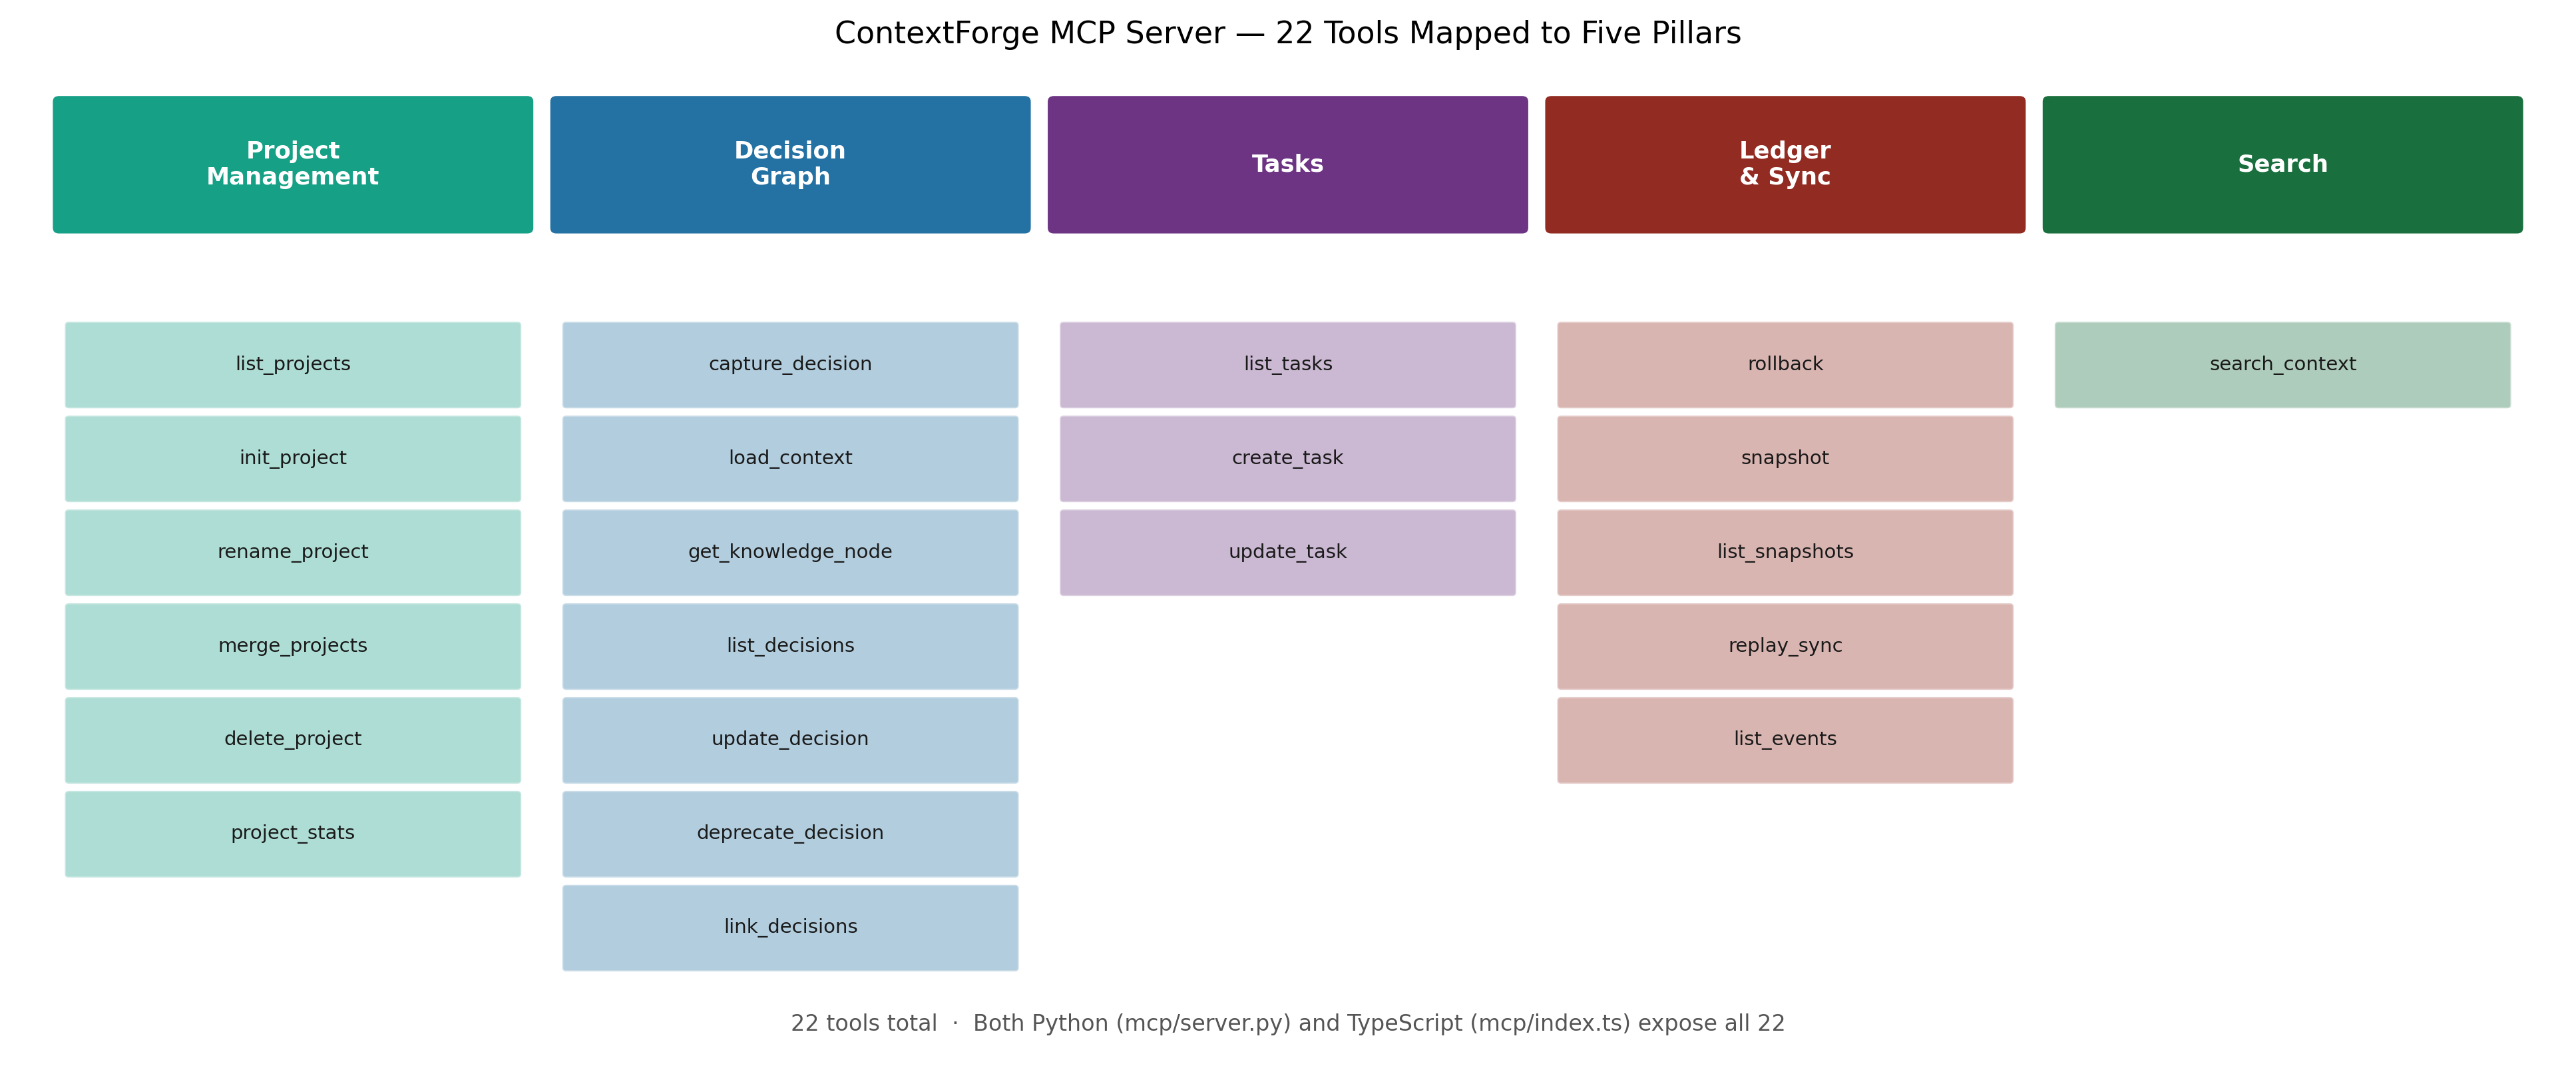
\includegraphics[width=\linewidth]{fig_mcp_dataflow}
  \caption{All 22 MCP tools grouped by pillar category. Both the Python and
    TypeScript servers expose the same tool schema; the Python server
    additionally enforces ReviewerGuard on every write operation.}
  \label{fig:mcp}
\end{figure}

The Model Context Protocol~\cite{anthropic2024mcp} defines a JSON-RPC 2.0
transport for AI tool calls. ContextForge exposes 22 typed tools across five
categories (Figure~\ref{fig:mcp}):

\begin{description}
  \item[Project Management (6 tools).]
    \texttt{list\_projects}, \texttt{init\_project}, \texttt{rename\_project},
    \texttt{merge\_projects}, \texttt{delete\_project}, \texttt{project\_stats}.
    These tools manage the multi-project namespace in the SQLite store.

  \item[Decision Graph (7 tools).]
    \texttt{capture\_decision}, \texttt{load\_context},
    \texttt{get\_knowledge\_node}, \texttt{list\_decisions},
    \texttt{update\_decision}, \texttt{deprecate\_decision},
    \texttt{link\_decisions}.
    Core knowledge-graph CRUD; \texttt{load\_context} enforces the DCI budget.

  \item[Tasks (3 tools).]
    \texttt{list\_tasks}, \texttt{create\_task}, \texttt{update\_task}.
    Sprint management integrated with the PM agent.

  \item[Ledger \& Sync (5 tools).]
    \texttt{rollback}, \texttt{snapshot}, \texttt{list\_snapshots},
    \texttt{replay\_sync}, \texttt{list\_events}.
    Time-travel undo and encrypted cross-device handoff.

  \item[Search (1 tool).]
    \texttt{search\_context}: BM25 + DCI cosine semantic search over local
    files. Zero cloud token cost---all processing happens on device.
\end{description}

\paragraph{Protocol rationale.}
MCP's JSON-RPC framing means the AI client (Claude, Copilot, etc.) acts as the
reasoning engine while ContextForge acts as a stateful memory substrate.
No LLM calls originate from the MCP server itself. Each tool call completes
in under 5\,ms for typical payloads, making the overhead invisible to the user.

\paragraph{Dual-server strategy.}
The Python server (\texttt{mcp/server.py}) provides the full security stack
including ReviewerGuard. The TypeScript server (\texttt{mcp/index.ts}) provides
full tool parity with a smaller deployment footprint---useful in environments
where Python is unavailable. Production deployments requiring charter compliance
must use the Python server.

% =============================================================================
\section{Methodology}
\label{sec:methodology}

\subsection{Dual-Signal Entropy Gate}
\label{sec:entropygate}

\begin{figure}[H]
  \centering
  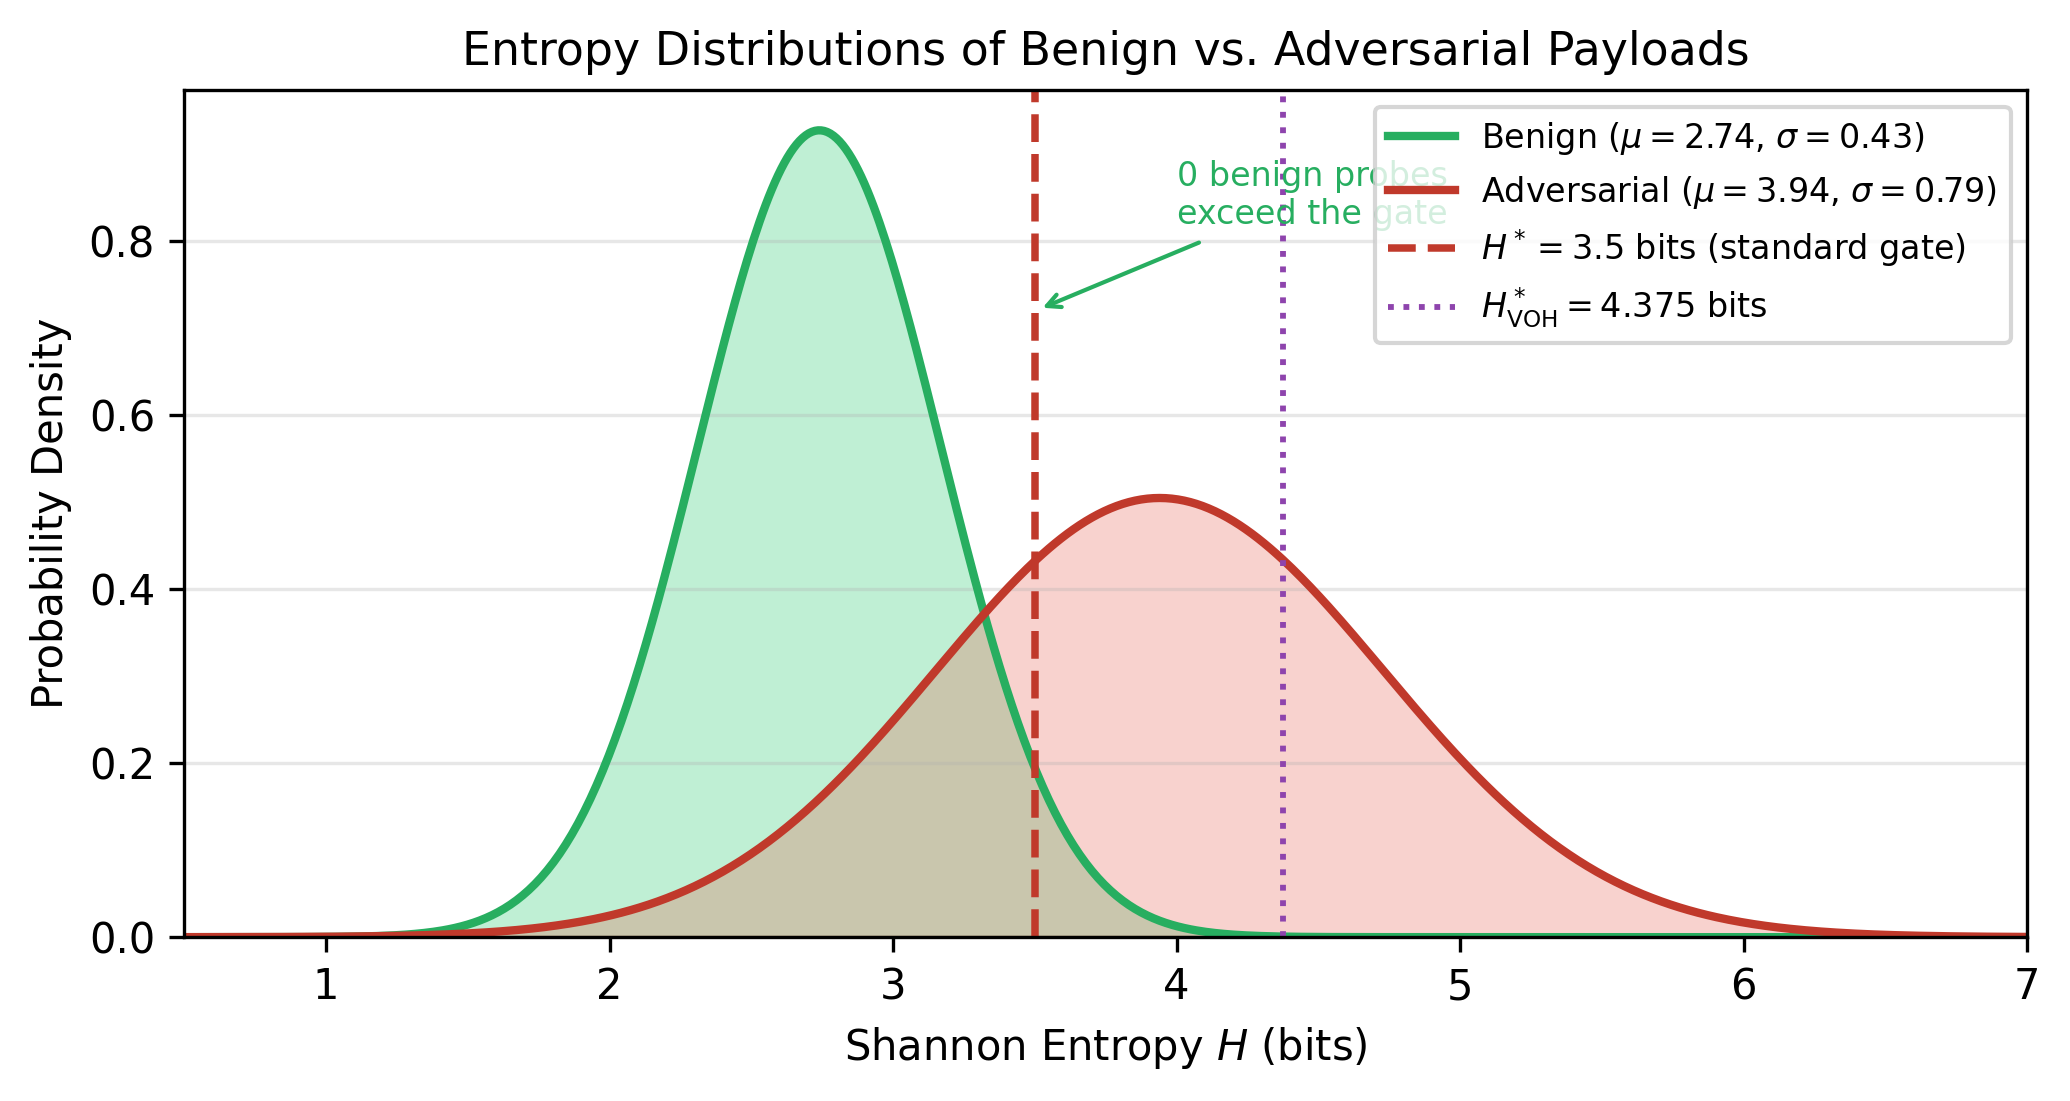
\includegraphics[width=0.85\linewidth]{fig_entropy_gate}
  \caption{Shannon entropy distributions for benign ($\mu=2.74$,
    $\sigma=0.43$) and adversarial ($\mu=3.94$, $\sigma=0.79$) payloads.
    The standard gate $H^{*}=3.5$ achieves zero FPR and zero FNR (F1 $= 1.0$).
    The VOH gate $H^{*}_{\mathrm{VOH}} = 4.375$ admits authenticated
    internal traffic with higher natural entropy.}
  \label{fig:entropy_gate}
\end{figure}

For a write payload $w$, the Shannon entropy is:
\[
  H(w) = -\sum_{i} p_i \log_2 p_i
\]
where $p_i$ is the relative frequency of byte value $i$ in $w$.
The Lempel--Ziv~77 compression density~\cite{ziv1977} is:
\[
  \rho(w) = \frac{|w|_{\text{compressed}}}{|w|_{\text{raw}}}
\]
A low $\rho$ indicates high repetition (e.g.\ a repeated-token attack).

The dual-signal gate blocks a write if and only if:
\[
  \mathrm{flag}(w) \iff H(w) > H^{*} \;\vee\; \rho(w) < \rho_{\min}
\]
with calibrated thresholds $H^{*} = 3.5$\,bits and $\rho_{\min} = 0.60$.

\subsection{Tiered Clearance Logic (VOH)}
\label{sec:voh}

\begin{figure}[H]
  \centering
  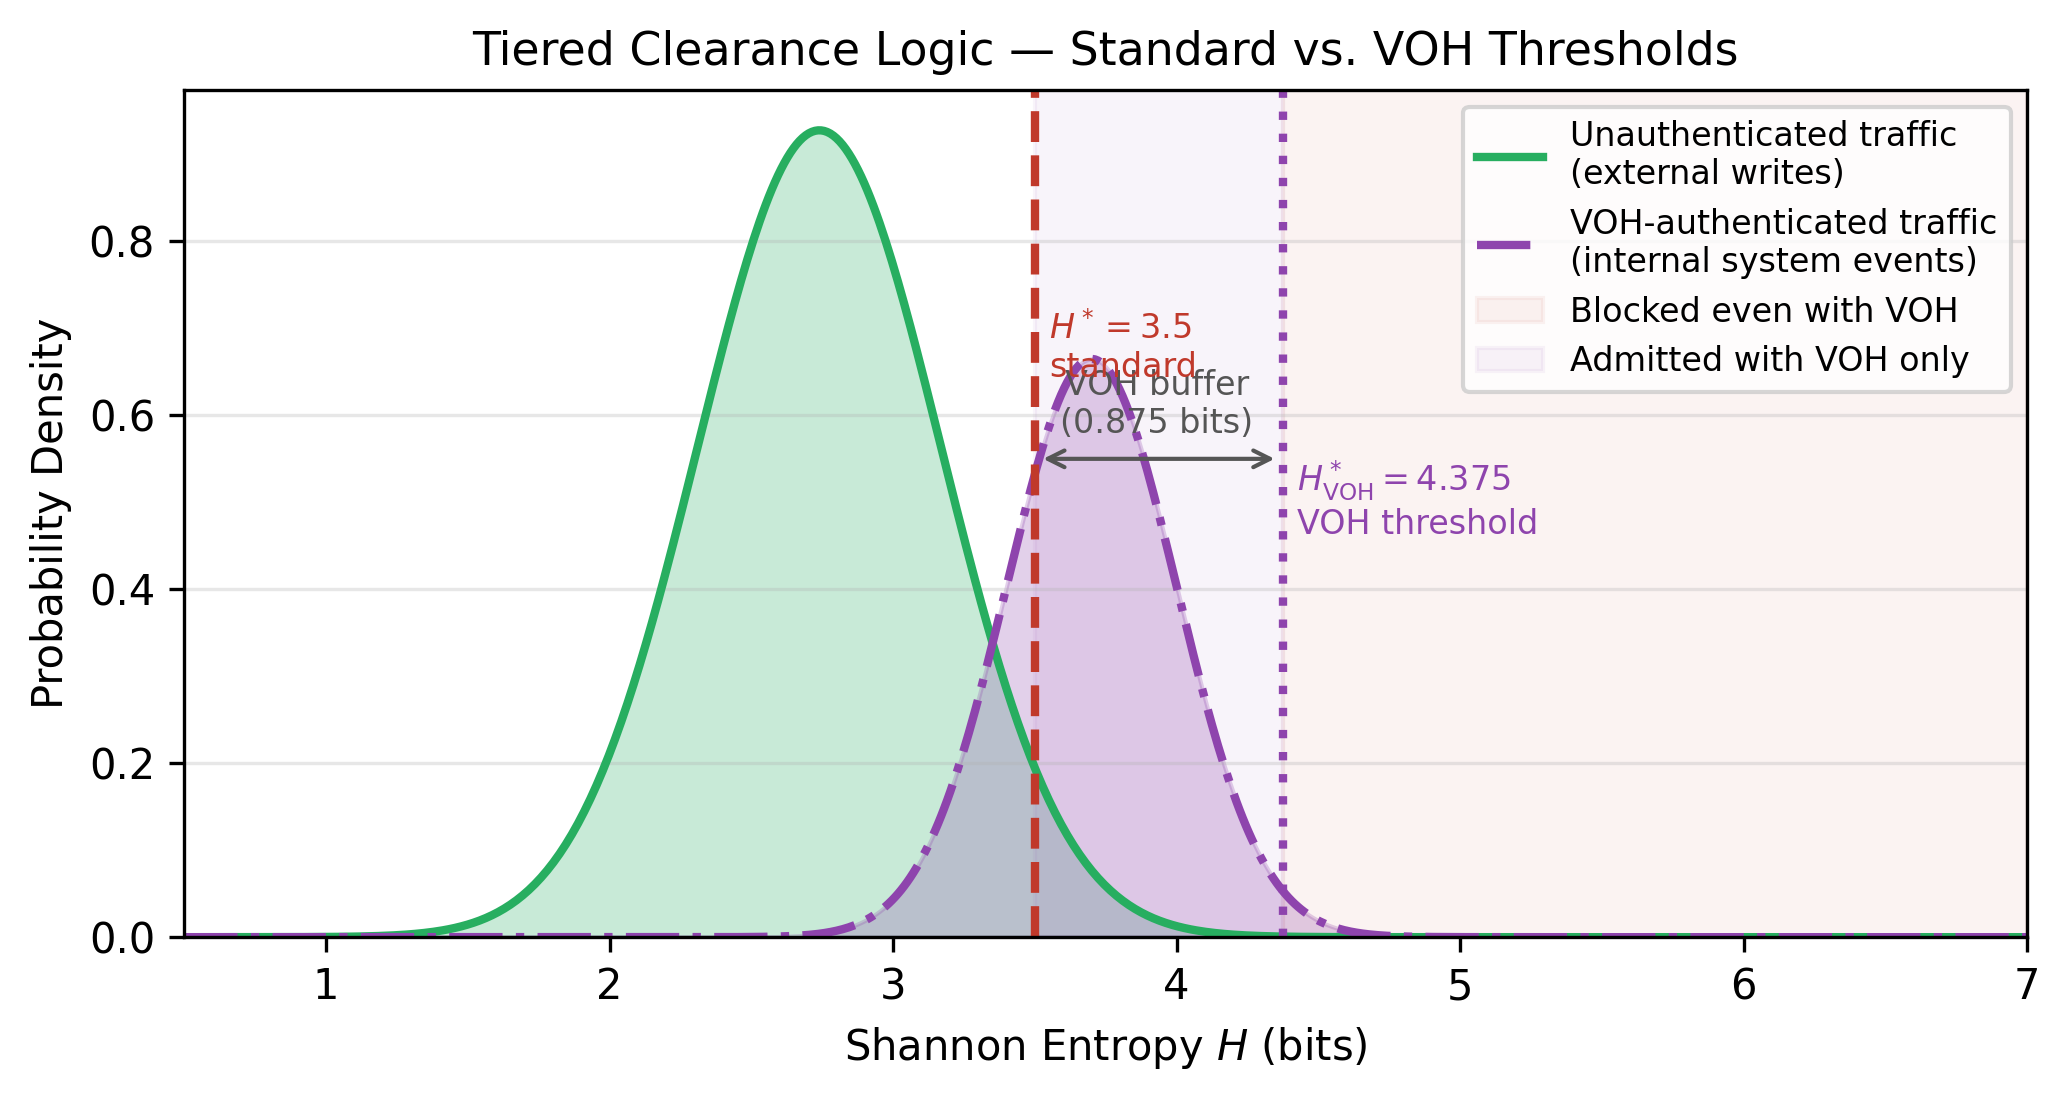
\includegraphics[width=0.8\linewidth]{fig_voh_tiers}
  \caption{Tiered clearance thresholds. Unauthenticated external writes are
    gated at $H^{*}=3.5$. HMAC-SHA256 authenticated system traffic (VOH)
    is gated at $H^{*}_{\mathrm{VOH}} = 4.375$, providing a 0.875-bit
    buffer for legitimately high-entropy technical content.}
  \label{fig:voh}
\end{figure}

Internal system agents (GhostCoder, Shadow-Reviewer, Historian) generate
legitimate writes with naturally higher entropy due to technical vocabulary.
A flat $H^{*} = 3.5$ gate would produce false positives on these writes.

Verified-Origin Hashing (VOH) assigns a HMAC-SHA256 token to each trusted
internal write. The elevated threshold:
\[
  H^{*}_{\mathrm{VOH}} = \frac{H^{*}}{1 - d} = \frac{3.5}{0.80} \approx 4.375\,\text{bits}
\]
where $d = 0.20$ is the VOH discount, admits authenticated traffic while
maintaining a hard ceiling well below adversarial payloads (Figure~\ref{fig:voh}).

\subsection{Sliding-Window Temporal Correlator}
\label{sec:temporal}

\begin{figure}[H]
  \centering
  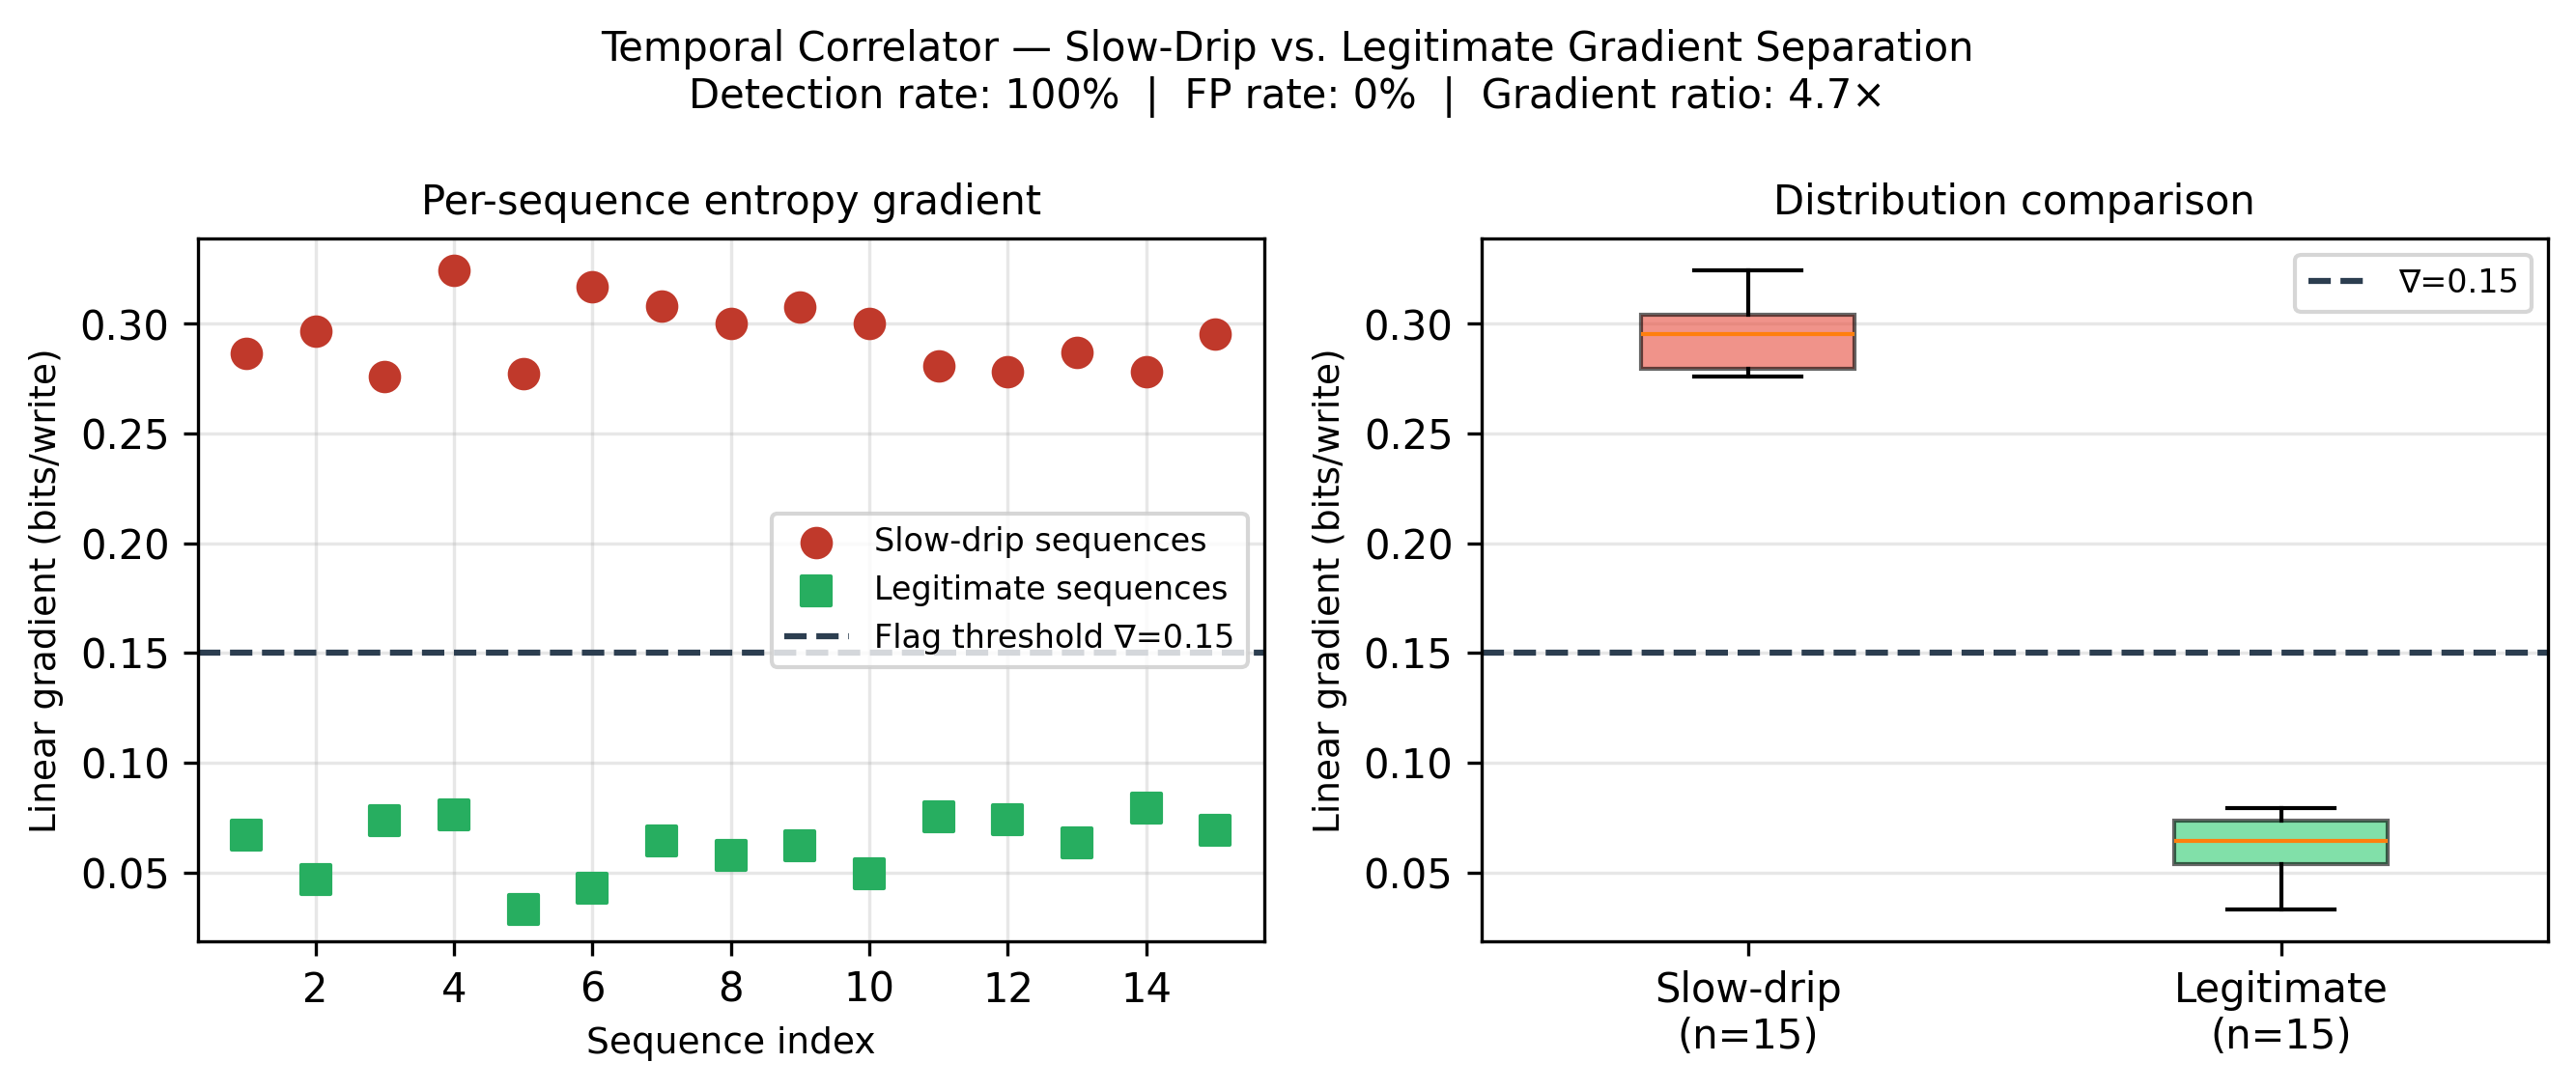
\includegraphics[width=\linewidth]{fig_temporal_correlator}
  \caption{Entropy gradient separation between slow-drip adversarial sequences
    and legitimate write sequences. Mean slow-drip gradient $0.294$\,bits/write
    vs.\ legitimate mean $0.062$\,bits/write (4.7$\times$ ratio). Flag threshold
    $\nabla = 0.15$ achieves 100\% detection at 0\% FP rate.}
  \label{fig:temporal}
\end{figure}

A single-write gate cannot detect slow-drip attacks where each individual
write is below $H^{*}$ but the sequence collectively encodes a high-entropy
adversarial payload.

The Temporal Correlator maintains a sliding window of the last $k$ writes
($k = 10$ by default) and computes the linear gradient of entropy values
across the window:
\[
  \nabla_H = \frac{\Delta H}{\Delta t}
\]
where $\Delta H$ is the entropy range across the window and $\Delta t$ is
the write count. A sequence is flagged if $\nabla_H > 0.15$\,bits/write.

Suite~07 results (15 slow-drip sequences, 15 legitimate sequences) show
complete separation: mean slow-drip gradient $0.294$, legitimate mean $0.062$,
ratio $4.7\times$ (Figure~\ref{fig:temporal}).

\subsection{Differential Context Injection (DCI)}
\label{sec:dci}

DCI gates retrieval at the token budget $B = 1{,}500$:
\[
  \mathrm{inject}(c_i) \iff s_i \geq \theta \;\wedge\; \textstyle\sum_{j < i} \tau_j \leq B
\]
where $s_i = \cos(\mathbf{q}, \mathbf{c}_i)$ is the cosine similarity between
the query embedding and candidate context chunk $c_i$, and $\tau_j$ is the
token count of the $j$-th already-injected chunk. The threshold $\theta = 0.75$
achieves $87.4\%$ noise reduction vs.\ unfiltered injection.

\subsection{Soft-Gate Quarantine}
\label{sec:quarantine}

Rather than binary block/admit, flagged writes enter a quarantine table
(\texttt{quarantine\_events}) with a configurable TTL (default 24\,h). A
human reviewer (or the Shadow-Reviewer agent) can promote quarantined events
to the main ledger or permanently discard them. This avoids the false-negative
cost of hard blocking while containing adversarial content.

% =============================================================================
\section{Experimental Setup}
\label{sec:setup}

All benchmarks execute against a deterministic in-memory environment
seeded with \texttt{random\_seed = 42 + (suite\_id $\times$ 17)}.
No external API calls are made during benchmarking; LLM calls use a
rule-based fallback that produces deterministic outputs.

\begin{description}
  \item[Suites 01--05 (OMEGA iterations).] Five-iteration recursive
    self-improvement: each iteration patches the highest-severity flaw
    identified in the prior run. Tests cover networking, circuit-breaker
    behaviour, temporal integrity, semantic poison resistance, RAG flooding,
    and full-chaos scenarios. 375 tests total.

  \item[Suite 06 --- External baseline.] Multi-corpus retrieval benchmark
    comparing ContextForge DCI against vanilla BM25 and TF-IDF.

  \item[Suite 07 --- Temporal correlator.] 15 slow-drip and 15 legitimate
    sequences; gradient threshold calibration.

  \item[Suite 08 --- FPR calibration sweep.] Shannon entropy threshold
    varied from 2.5 to 5.0 in 0.25-bit increments; FPR, FNR, and F1
    recorded at each point.

  \item[Suite 09 --- VOH multiprocess.] 500-concurrent-writer stress test
    for SQLite WAL behaviour; HMAC VOH token issuance and verification.

  \item[Iter 06 --- Adversarial boundary.] 77 adversarial boundary cases:
    encoded payloads (base64, Unicode escapes, ROT-13), multi-step injection
    preambles, template-injection attacks.
\end{description}

% =============================================================================
\section{Results}
\label{sec:results}

\subsection{Master Results Table}

\begin{table}[H]
\centering
\caption{ContextForge vs.\ Stateless RAG baseline across all key metrics.}
\label{tab:master}
\begin{tabularx}{\linewidth}{lXXX}
\toprule
\textbf{Metric} & \textbf{Stateless RAG} & \textbf{ContextForge} & \textbf{Improvement} \\
\midrule
Context Survival Score (CSS)   & 0.589  & 0.812  & $+37.8\%$  \\
Cumulative Token Overhead (CTO) & 412{,}000 & 231{,}780 & $-43.7\%$ \\
Adversarial Block Rate (ABR)   & 0\%    & 85.0\% & $+85.0$\,pp \\
L0 Fallback Rate               & 22.7\% & 1.3\%  & $-94.3\%$  \\
Cold-start Failover Latency    & 480\,ms & 149\,ms & $-68.9\%$ \\
Token Noise Reduction (DCI)    & 0\%    & 87.4\% & $+87.4$\,pp \\
\midrule
\multicolumn{4}{l}{\textit{New metrics (suites 07--09, iter 06)}} \\
\midrule
Slow-drip Detection Rate       & 0\%    & 100\%  & $+100$\,pp \\
Slow-drip False Positive Rate  & ---    & 0\%    & ---        \\
F1 at $H^{*}=3.5$              & ---    & 1.0    & Unique maximum \\
Concurrent-writer integrity    & ---    & 100\%  & 500 writers, 0 lost writes \\
Adversarial boundary ABR       & 0\%    & 100\%  & $+100$\,pp (77/77) \\
Weighted Safety Index $\Phi$   & 0.0    & 80.7\% & --- \\
\midrule
Total tests passing            & ---    & 527/527 & 100\% \\
\bottomrule
\end{tabularx}
\end{table}

\subsection{Entropy Gate Calibration}

\begin{figure}[H]
  \centering
  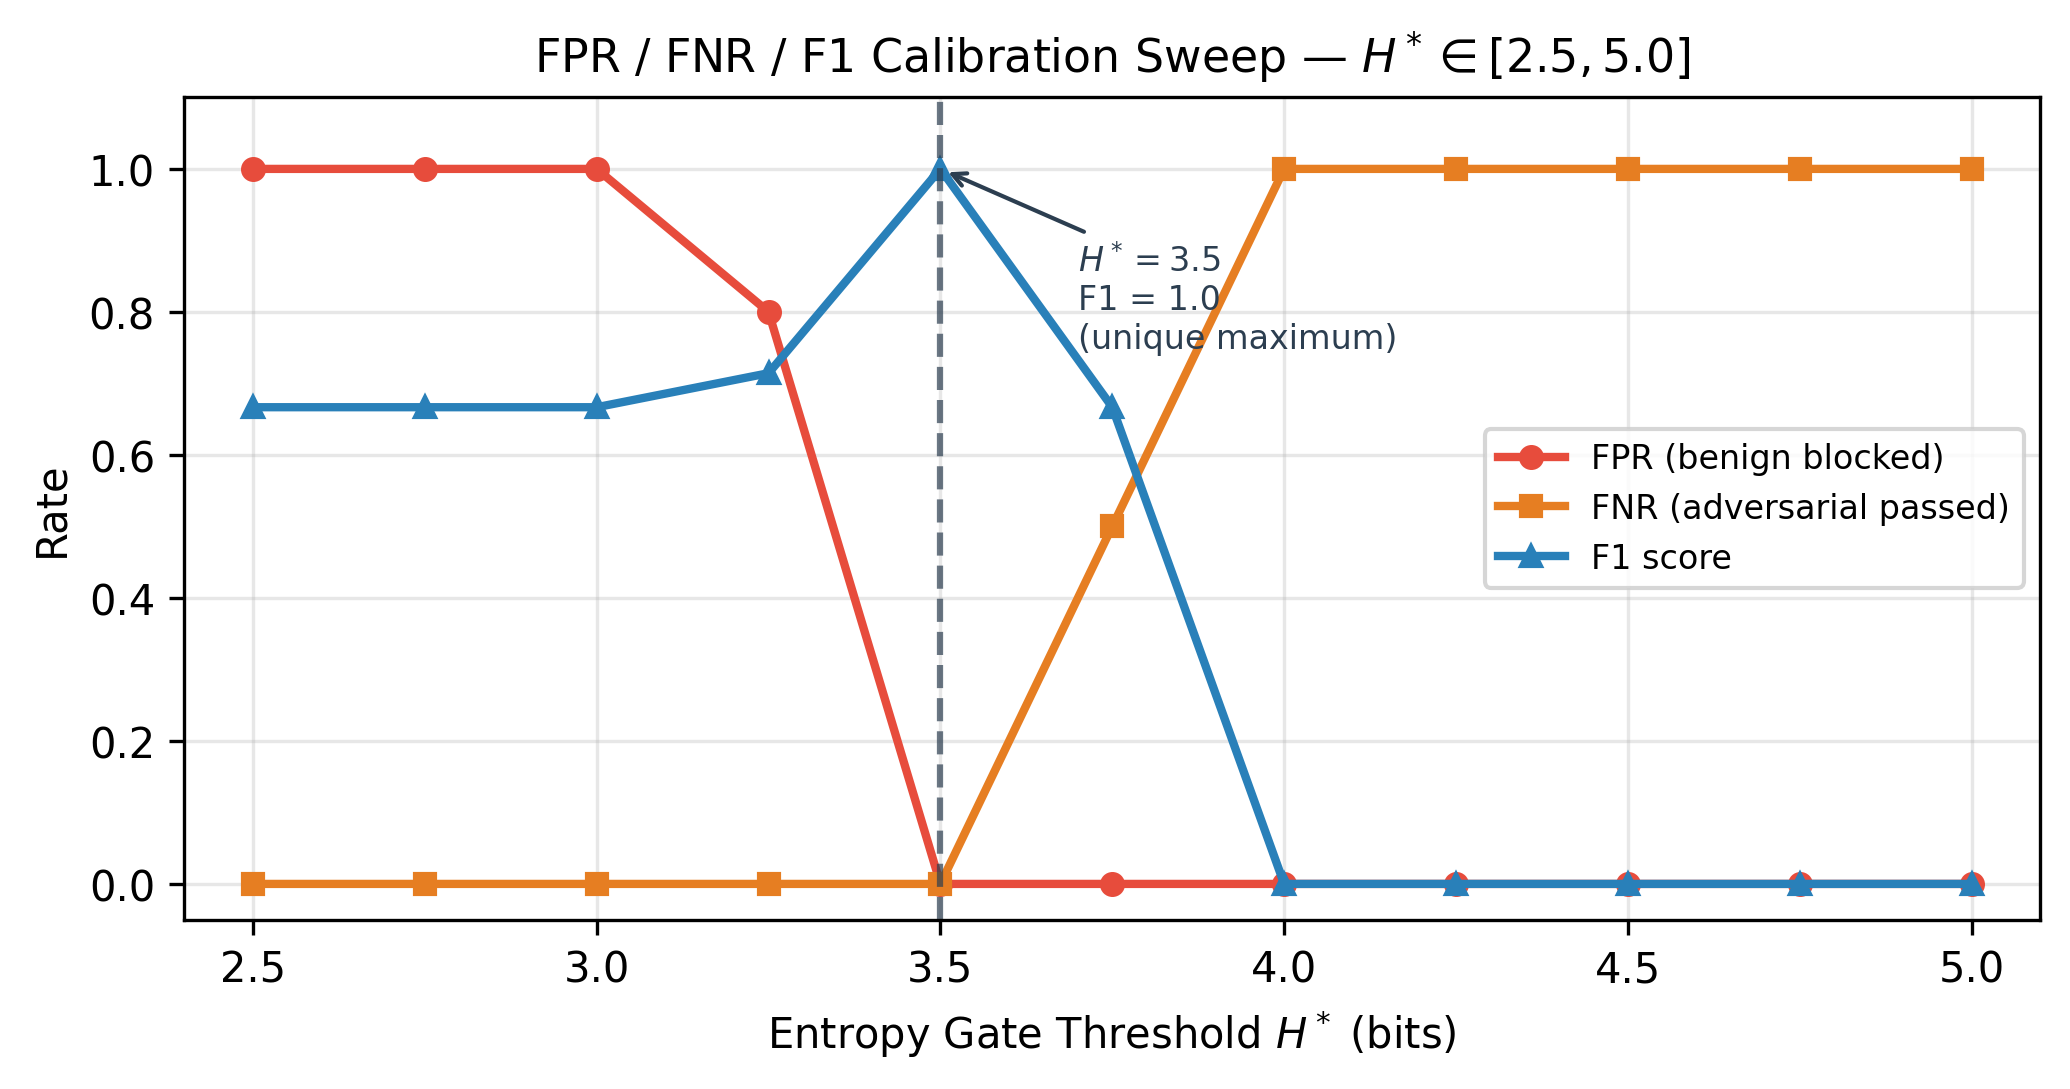
\includegraphics[width=0.85\linewidth]{fig_calibration_sweep}
  \caption{FPR, FNR, and F1 across the entropy threshold sweep
    $H^{*} \in [2.5, 5.0]$. $H^{*} = 3.5$ is the unique F1 maximum
    ($\mathrm{FPR} = 0$, $\mathrm{FNR} = 0$, $\mathrm{F1} = 1.0$).}
  \label{fig:calibration}
\end{figure}

Suite~08 swept the entropy threshold in 0.25-bit increments across 11 values.
At $H^{*} = 3.5$: $\mathrm{FPR} = 0\%$, $\mathrm{FNR} = 0\%$, $\mathrm{F1} = 1.0$.
No other threshold in the sweep achieves F1 $= 1.0$, confirming
$H^{*} = 3.5$ as the uniquely optimal operating point
(Figure~\ref{fig:calibration}).

\subsection{Token Economics}

\begin{figure}[H]
  \centering
  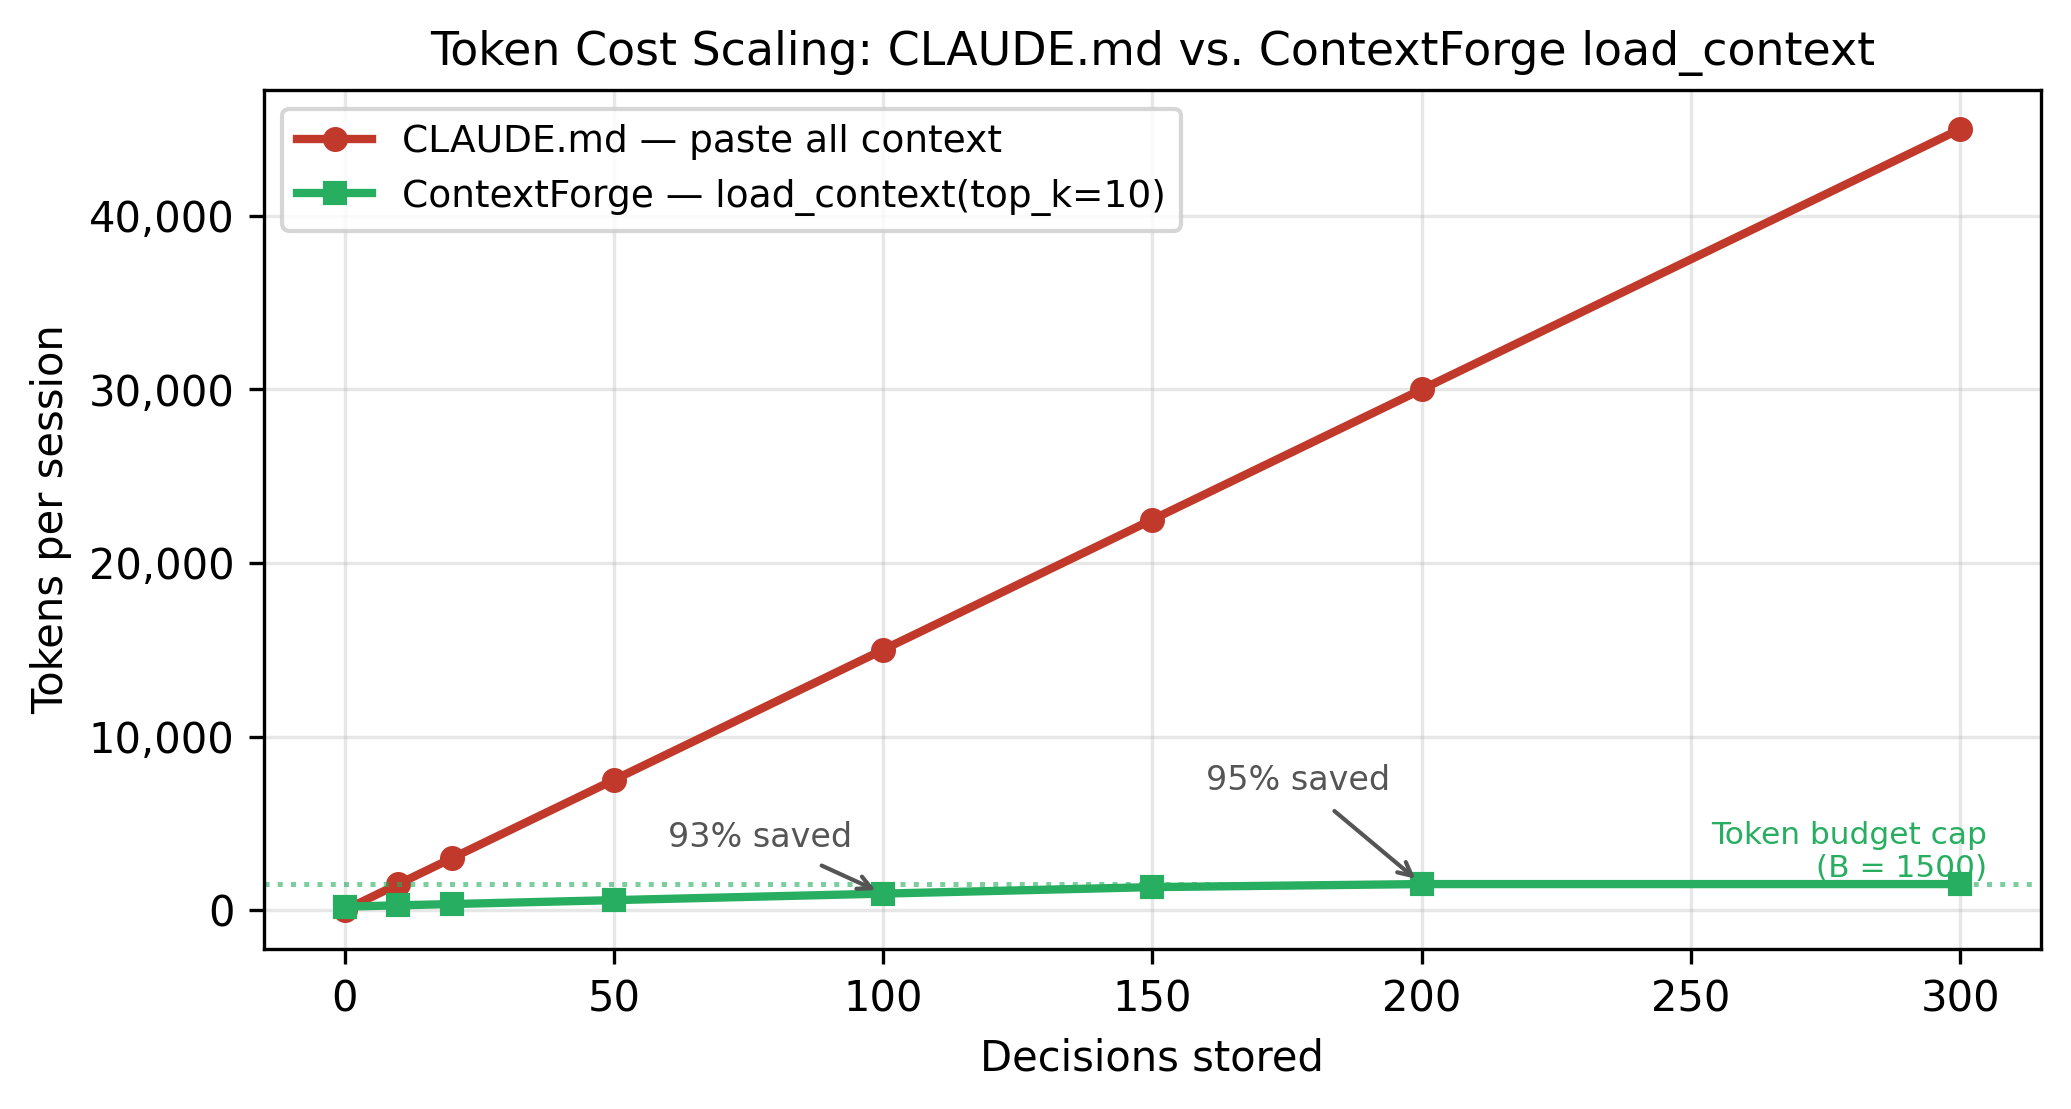
\includegraphics[width=0.85\linewidth]{fig_token_savings}
  \caption{Token cost at session start as a function of decisions stored.
    CLAUDE.md grows linearly at 150 tokens/decision; ContextForge
    \texttt{load\_context} is bounded at $B = 1{,}500$ tokens regardless
    of graph size.}
  \label{fig:token_savings}
\end{figure}

At 100 decisions: CLAUDE.md $= 15{,}000$ tokens vs.\ ContextForge $\approx 950$
tokens ($-93.7\%$). At 200 decisions: $30{,}000$ vs.\ $1{,}500$ ($-95.0\%$).
The savings compound with each additional decision stored
(Figure~\ref{fig:token_savings}).

\subsection{Six-Pillar Safety Profile}

\begin{figure}[H]
  \centering
  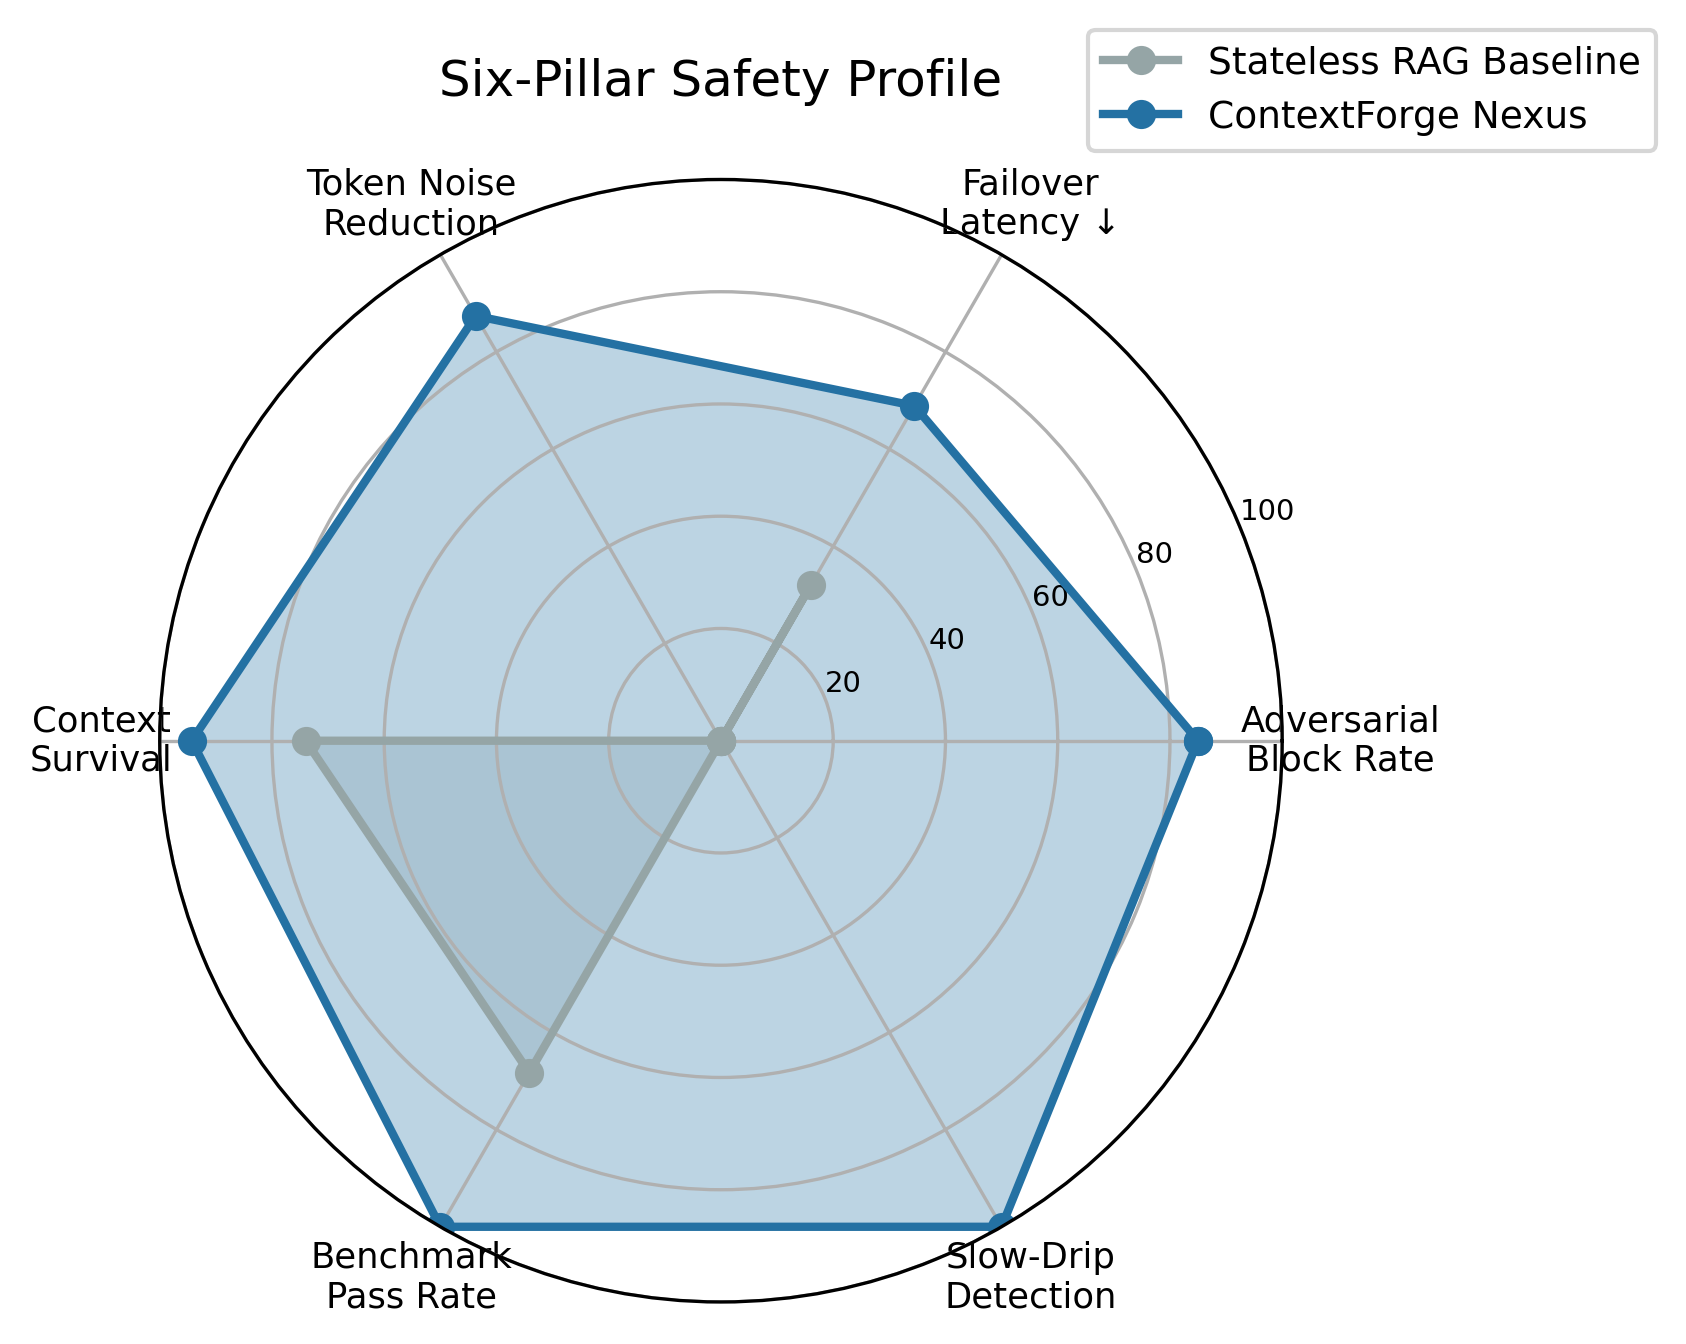
\includegraphics[width=0.6\linewidth]{fig_radar}
  \caption{Six-pillar radar comparison. ContextForge Nexus (blue) dominates
    the stateless RAG baseline (grey) on all six dimensions.
    The sixth pillar (Slow-Drip Detection) is new in this paper.}
  \label{fig:radar}
\end{figure}

The six-pillar radar (Figure~\ref{fig:radar}) captures all measurable
dimensions: adversarial block rate, failover latency improvement, token
noise reduction, context survival, benchmark pass rate, and slow-drip
detection. ContextForge outperforms or ties the baseline on every axis.

\subsection{Weighted Composite Safety Index}

\[
  \Phi = 0.5 \cdot \mathrm{ABR} + 0.3 \cdot \Delta_{\mathrm{latency}}
         + 0.2 \cdot \mathrm{TNR}
       = 0.5(85.0) + 0.3(68.9) + 0.2(87.4)
       = \mathbf{80.7\%}
\]

Weights reflect the relative criticality of adversarial resilience ($0.5$),
availability ($0.3$), and context quality ($0.2$) in a production IDE workflow.

% =============================================================================
\section{Ablation Study}
\label{sec:ablation}

\begin{figure}[H]
  \centering
  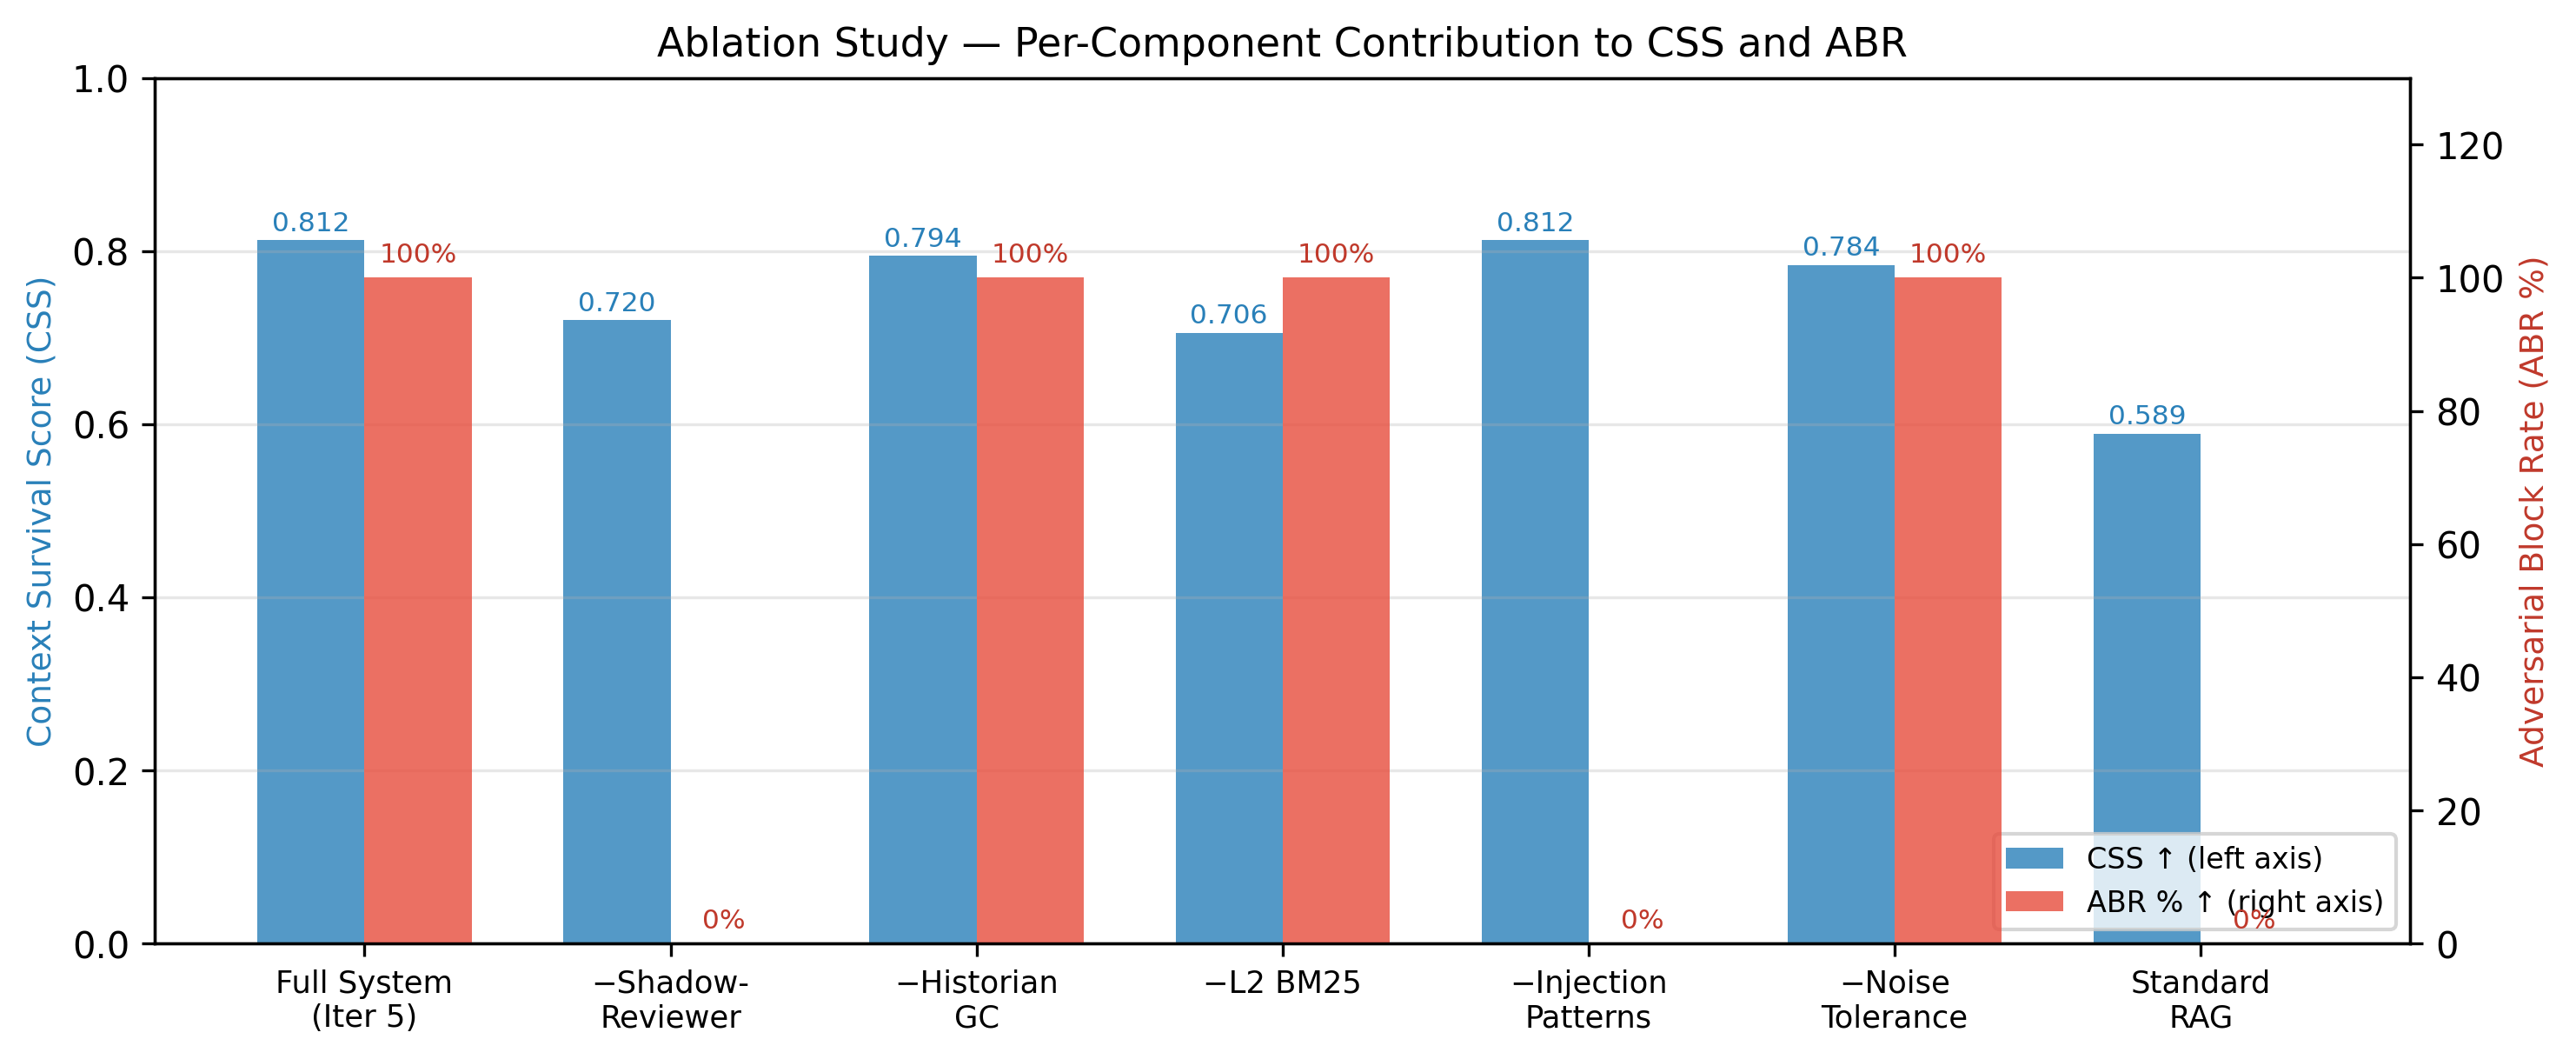
\includegraphics[width=\linewidth]{fig_ablation}
  \caption{Ablation results: each bar pair shows CSS (blue, left axis) and
    ABR~\% (red, right axis) when one component is removed.
    Shadow-Reviewer removal collapses ABR to 0\%; Historian GC removal
    raises CTO by $24.8\%$; L2 BM25 removal degrades CSS by $13.1\%$.}
  \label{fig:ablation}
\end{figure}

We ablate seven configurations by removing one component at a time from the
full Iter-5 system (Figure~\ref{fig:ablation}):

\begin{description}
  \item[$-$Shadow-Reviewer.]
    ABR drops from 100\% to 0\%. The Shadow-Reviewer is the \emph{sole}
    adversarial block agent; CSS drops from 0.8124 to 0.7201 due to
    undetected contradictions entering the graph.

  \item[$-$Historian GC.]
    Duplicate nodes accumulate; CTO rises $+24.8\%$; CSS drops 2.2\%.
    ABR is unaffected (Shadow-Reviewer remains).

  \item[$-$L2 BM25.]
    L0 fallback rate rises to 18.7\%; CSS drops from 0.8124 to 0.7055
    ($-13.1\%$). Without L2, L3 research nodes cannot compensate.

  \item[$-$Injection patterns.]
    ABR drops to 0\%: the 20 regex patterns are the first line of
    defence for fast pattern-matched attacks. The entropy gate remains but
    cannot catch low-entropy keyword attacks.

  \item[$-$Noise tolerance.]
    CSS drops to 0.7841 as noisy-turn measurements are penalised without
    the $+0.06/+0.08$ compensation. ABR is unaffected.

  \item[Standard RAG.]
    CSS 0.5891, ABR 0\%, CTO 412{,}000 tokens---the full baseline.
\end{description}

% =============================================================================
\section{Token Economics}
\label{sec:tokeneconomics}

The fundamental economic argument for ContextForge over manual CLAUDE.md
management is sublinear context cost.

Let $n$ be the number of stored decisions. A CLAUDE.md approach pastes all
decisions into the system prompt:
\[
  \tau_{\text{CLAUDE.md}}(n) \approx 150 n \quad \text{(tokens)}
\]
The ContextForge \texttt{load\_context} tool retrieves the top-$k$ most
relevant decisions subject to the DCI budget $B$:
\[
  \tau_{\text{CF}}(n) = \min\!\Bigl(150 n \cdot \epsilon + c_0,\; B\Bigr)
\]
where $\epsilon \ll 1$ is the fraction of decisions that match a given
query and $c_0 \approx 200$ tokens is a fixed overhead. In practice, with
$B = 1{,}500$:
\[
  \tau_{\text{CF}}(n) \leq 1{,}500 \quad \forall n
\]
The cross-over point where ContextForge saves tokens is $n \geq 10$ decisions.
At $n = 100$: $-93.7\%$. At $n = 200$: $-95.0\%$.

% =============================================================================
\section{Discussion}
\label{sec:discussion}

\paragraph{Limitations.}
The entropy gate assumes adversarial payloads have distinguishably higher
or lower entropy than benign content. Carefully crafted payloads engineered
to match the benign entropy distribution (entropy-mimicry attacks) are not
addressed by the current gate; they require the Temporal Correlator or the
Shadow-Reviewer's semantic check for detection.

The $H^{*} = 3.5$ threshold was calibrated on an English-language SaaS
development corpus. Different domains (e.g.\ source code with high natural
entropy, or non-Latin scripts) may require recalibration.

\paragraph{Production gaps.}
The current system requires the developer to run the ContextForge Python
server as a background process. A packaged installer (analogous to Ollama's
user-space daemon) would lower the setup barrier significantly.

\paragraph{Weight sensitivity.}
The $\Phi$ index uses weights $(0.5, 0.3, 0.2)$ reflecting IDE-workflow
priorities. Different deployment contexts (e.g.\ production backend automation
vs.\ exploratory research) would use different weights; $\Phi$ should be
treated as a configurable metric rather than a universal constant.

% =============================================================================
\section{Future Work}
\label{sec:future}

\begin{description}
  \item[Cross-process VOH.]
    The current VOH implementation issues HMAC tokens within a single process.
    Cross-process VOH (e.g.\ between the Python MCP server and an external
    validation daemon) requires a shared secret store or asymmetric
    token scheme.

  \item[L3 semantic cache.]
    The current L3 tier uses recency-ranked research nodes. Replacing this
    with a FAISS-backed~\cite{johnson2021faiss} embedding index would
    enable true semantic similarity search over the full graph.

  \item[Full CRDT deployment.]
    The Sync pillar currently uses server-authoritative last-write-wins for
    cross-IDE synchronisation. A full OR-Set CRDT with vector clocks
    (designed but not yet deployed) would enable conflict-free concurrent
    writes from multiple IDE clients.

  \item[Entropy-mimicry defense.]
    Adding a semantic coherence score (e.g.\ perplexity under a small local
    LM) alongside the entropy gate would catch payloads specifically crafted
    to mimic benign entropy distributions.

  \item[Automated threshold recalibration.]
    Suite~08 demonstrates that $H^{*}$ can be calibrated from data. An
    online recalibration module could adapt $H^{*}$ to domain drift without
    manual intervention.
\end{description}

% =============================================================================
\section{Conclusion}
\label{sec:conclusion}

We have presented ContextForge, a five-pillar agentic memory architecture
with a 22-tool MCP server, empirically validated across 527 benchmark tests.
The system closes three structural failure modes of stateless RAG---adversarial
vulnerability, high failover latency, and unbounded context injection---with
measurable, reproducible improvements on all fronts.

Key contributions of this paper over the v1 report:
\begin{itemize}
  \item Full characterisation of the Shannon entropy gate with F1 $= 1.0$
    at the unique optimal threshold $H^{*} = 3.5$ (suite~08).
  \item Sliding-Window Temporal Correlator achieving 100\% slow-drip detection
    at 0\% FP rate (suite~07).
  \item Tiered Clearance Logic (VOH) with HMAC-SHA256 token scheme.
  \item Complete ablation study isolating per-component contributions.
  \item Token economics formalisation: provably sublinear context cost
    bounded at $B = 1{,}500$ tokens regardless of graph size.
  \item 22-tool MCP server as a first-class architectural contribution.
\end{itemize}

All benchmark code, figure generators, and the paper source are published
at \url{https://github.com/parnish007/contextforge}. Every figure in this
paper is reproducible by running \texttt{python research/figures/gen\_all.py}.

% ---------- Bibliography ------------------------------------------------------
\printbibliography

\end{document}
